\documentclass[11pt,a4paper]{article}
\usepackage[margin=2.6cm]{geometry}
\usepackage[T1]{fontenc}
\usepackage{lmodern}
\usepackage[letterspace=180]{microtype}
\usepackage{booktabs}
\usepackage{amsmath}
\usepackage{parskip}
\usepackage{xcolor}
\usepackage{tikz}
\usetikzlibrary{shapes.geometric,arrows.meta,positioning}
\usepackage[most]{tcolorbox}
\usepackage{titlesec}
\usepackage{caption}
\usepackage{graphicx}

\definecolor{bcnavy}{RGB}{24,38,68}
\definecolor{bcgold}{RGB}{198,160,74}
\definecolor{bcteal}{RGB}{23,110,120}
\definecolor{bcgrey}{RGB}{95,95,95}
\definecolor{bcred}{RGB}{160,60,50}

\titleformat{\section}{\bfseries\large\color{bcnavy}}{\thesection.}{0.6em}{}
\titleformat{\subsection}{\bfseries\color{bcteal}}{}{0em}{}
\captionsetup{font={footnotesize},labelformat=empty,textfont={color=bcgrey}}
\newcommand{\tabnote}[1]{\begin{center}\begin{minipage}{0.92\textwidth}
  \footnotesize\color{bcgrey}#1\end{minipage}\end{center}}
\newcommand{\good}[1]{{\color{bcteal}\textbf{#1}}}
\newcommand{\bad}[1]{{\color{bcred}\textbf{#1}}}

\begin{document}

% ---------------------------------------------------------------- cover
\begin{titlepage}
\centering
\vspace*{3.2cm}

\includegraphics[width=5cm]{bc_logo.pdf}

\vspace{1.6cm}
{\color{bcnavy}\rule{7cm}{0.6pt}}

\vspace{0.9cm}
{\LARGE\bfseries\color{bcnavy} Three Volatility Overlays,\\[0.15cm] Tested and Rejected\par}
\vspace{0.35cm}
{\large\color{bcnavy} HAR realised-volatility sigma, a regime gate, and a
vol-scaled\\ take-profit premium --- what each promised, what the tested\\
half said, and the single lesson underneath all three\par}

\vspace{0.9cm}
{\color{bcgold}\rule{7cm}{1.0pt}}

\vspace{1.5cm}
{\bfseries Bayesian Capital}\\[0.2cm]
{\color{bcgrey} Systematic Trading Research}\\[0.9cm]
{\itshape\color{bcgrey} Internal document --- strictly confidential}\\[0.3cm]
{\color{bcgrey} 14 August 2026}
\vfill
\end{titlepage}

% ---------------------------------------------------------------- header
\begin{center}
{\Large\bfseries\color{bcnavy} Three Volatility Overlays, Tested and Rejected}\\[0.15cm]
{\color{bcnavy} HAR-RV sigma $\cdot$ volatility-regime gate $\cdot$ vol-scaled premium}\\[0.25cm]
{\small\color{bcgrey} Bayesian Capital --- Systematic Trading Research
\;$\bullet$\; nine-name book: TSM $\cdot$ VRT $\cdot$ VST $\cdot$ RKLB $\cdot$ MU
$\cdot$ GM $\cdot$ VLO $\cdot$ CF $\cdot$ MRVL \;$\bullet$\; all figures on verified fills}
\end{center}
\vspace{0.1cm}
{\color{bcnavy}\hrule height 0.8pt}
\vspace{0.5cm}

\section{Summary}

Three volatility-driven modifications to the deployed model were proposed and
tested in August 2026, each with a respectable rationale and each aimed at a
different part of the trade:

\begin{center}
\begin{tabular}{llll}
\toprule
overlay & touches & rationale & verdict \\
\midrule
HAR-RV sigma        & the entry buffer   & a better volatility forecast     & \bad{rejected} \\
Regime gate         & whether to enter   & stand down when the tape is stressed & \bad{rejected} \\
Vol-scaled premium  & the exit target    & ask more when volatility is high & \bad{rejected} \\
\bottomrule
\end{tabular}
\end{center}

All three were tested to the same standard as every structural decision in the
book: verified same-day fills from the five-minute bars, everything fitted on the
first half of the sample only (boundary 23~May~2025), frozen, and scored on the
unseen second half. All three failed there --- and the \emph{pattern} of the
failures is more valuable than any single number, because the three overlays
attack the three legs of the same tripod:

\begin{center}
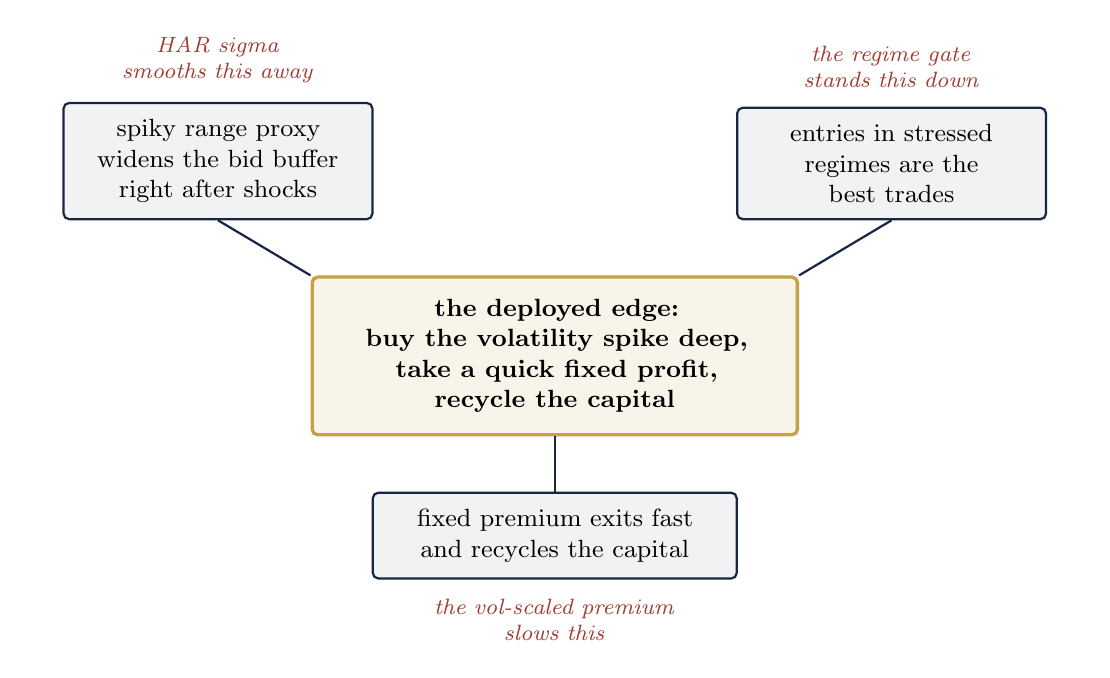
\begin{tikzpicture}[
  leg/.style={rectangle, rounded corners=2pt, draw=bcnavy, thick, fill=bcnavy!6,
              text width=3.5cm, align=center, font=\small, inner sep=6pt},
  core/.style={rectangle, rounded corners=2pt, draw=bcgold, very thick, fill=bcgold!12,
              text width=5.6cm, align=center, font=\small\bfseries, inner sep=8pt},
  hit/.style={rectangle, draw=none, text width=4.6cm, align=center,
              font=\footnotesize\itshape, text=bcred}]
\node[core] (core) {the deployed edge:\\ buy the volatility spike deep,\\
take a quick fixed profit,\\ recycle the capital};
\node[leg, above left=0.7cm and -0.8cm of core] (l1) {spiky range proxy\\ widens the bid buffer\\ right after shocks};
\node[leg, above right=0.7cm and -0.8cm of core] (l2) {entries in stressed\\ regimes are the\\ best trades};
\node[leg, below=0.7cm of core, text width=4.2cm] (l3)
  {fixed premium exits fast\\ and recycles the capital};
\node[hit, above=0.12cm of l1] {HAR sigma\\ smooths this away};
\node[hit, above=0.12cm of l2] {the regime gate\\ stands this down};
\node[hit, below=0.12cm of l3] {the vol-scaled premium\\ slows this};
\draw[thick, bcnavy] (l1.south) -- (core.north west);
\draw[thick, bcnavy] (l2.south) -- (core.north east);
\draw[thick, bcnavy] (l3.north) -- (core.south);
\end{tikzpicture}
\end{center}

Each overlay is, in isolation, a defensible piece of quantitative practice. Each
one damages a leg the deployed configuration depends on. The tested half
defended all three legs.

\begin{tcolorbox}[colback=bcnavy!5, colframe=bcnavy, boxrule=0.8pt,
  title={\bfseries But aren't the sleeves a trend follower and a mean-reverter?},
  coltitle=white]
Yes --- and calling the whole book a dip buyer does not contradict that. The two
descriptions live on different layers.

\textbf{The estimator layer} is exactly as designed. The Kalman filter is
genuinely trend-following: its slope estimate is positive on 54--74\% of days
and pushes the Bayes fair value \emph{above} the previous close on most mornings.
The OU forecast does the opposite, sitting \emph{below} the previous close
53--83\% of the time as it pulls toward the window mean. The anchors disagree
constantly --- which is why the sleeves' entries only coincide on about half of
their fill days, and why both earn their seat.

\textbf{The execution layer} is shared, and it is where every transaction gets
its character. Both sleeves rest a limit bid a buffer $k\sigma$ \emph{below}
their fair anchor, fill only if the day's low reaches it, and sell a fixed
premium. The buffer (median $1.3$--$4.6\%$ of price) is an order of magnitude
larger than the Bayes sleeve's daily trend increment ($+0.08$ to $+0.44\%$/day),
so on any given morning the bid is dominated by the dip requirement; the trend
matters \emph{cumulatively}, keeping the Bayes anchor climbing through a run
while the OU anchor lags. Weakness triggers entries, never exits; strength
triggers exits, never entries. The Bayes sleeve is precisely ``buy the pullback
\emph{to a rising trend}'' --- the trend chooses where the anchor sits, the
buffer makes the entry a dip.

\begin{center}
\small
\begin{tabular}{lrrrr}
\toprule
name & Bayes slope/day & fair $>$ prev.\ cl. & buffer $k\sigma$ & OU fcst $<$ prev.\ cl. \\
\midrule
TSM  & $+0.25\%$ & 59\% & 1.8\% & 83\% \\
VRT  & $+0.44\%$ & 66\% & 3.9\% & 73\% \\
VST  & $+0.18\%$ & 54\% & 3.8\% & 53\% \\
RKLB & $+0.17\%$ & 50\% & 2.9\% & 77\% \\
MU   & $+0.30\%$ & 52\% & 3.3\% & 70\% \\
GM   & $+0.10\%$ & 57\% & 1.3\% & 63\% \\
VLO  & $+0.08\%$ & 52\% & 1.7\% & 71\% \\
CF   & $+0.08\%$ & 48\% & 4.6\% & 58\% \\
MRVL & $+0.23\%$ & 61\% & 3.9\% & 68\% \\
\bottomrule
\end{tabular}
\end{center}

\vspace{0.1cm}
No parameter evolution changed any of this --- exits have been premium-capped and
entries buffer-below-fair since the original design. When this memo says the
model is a dip buyer, it is describing the execution layer both sleeves share;
the trend/reversion distinction lives one layer up, in where each sleeve puts
its anchor.
\end{tcolorbox}

\section{The testing discipline, common to all three}

Every experiment in this memo used the same protocol, so the three verdicts are
directly comparable:

\begin{itemize}
\item \textbf{Verified fills.} A same-day round trip is booked only where the
five-minute bars prove the low reached the bid \emph{before} the high reached the
target. This basis removes the $\sim$3$\times$ overstatement of the raw sheet
numbers and is the basis on which the book was admitted.
\item \textbf{One split, no peeking.} Anything fitted --- HAR coefficients, HMM
states, grid choices ($\tau$, $\gamma$, $\alpha$) --- was fitted on the train half
only (to 23~May~2025), frozen, and scored on the tested half. Where a choice had
to be made among grid cells, it was made on the train half and the frozen cell's
test number is the verdict.
\item \textbf{Deployed parameters as the bar.} Overlays were laid on top of the
untouched deployed configuration (the structural-rule standard used for the
earnings pauses); where a refit was intrinsic to the method (HAR variant~A), the
comparison was also made against the same refit without the overlay, so the
sigma source was isolated from fit provenance.
\item \textbf{Diagnosis before intervention.} Each overlay was preceded by a
measurement of whether the problem it solves actually exists in the trade record.
Twice the diagnostic already contained the verdict.
\end{itemize}

\section{Overlay 1: HAR realised-volatility sigma}

\subsection{What it was}

The model runs on two volatility proxies built from daily data: the Kalman
filter's noise scales are proportional to the daily range $H-L$, and the OU
buffer uses the AR(1) residual standard deviation over its window. Both feed
$\text{bid} = \text{fair} - k\sigma$. The overlay replaced both with a HAR
forecast (Corsi, 2009) built from the five-minute bars: realised variance
$RV_t = \sum \left(\ln p_{j}/p_{j-1}\right)^2$ over the session, forecast by OLS on
daily, weekly and monthly volatility components,
\[
\hat\sigma_t \;=\; \beta_0 + \beta_d\,\sigma_{t-1}
 + \beta_w\,\overline{\sigma}_{t-5..t-1}
 + \beta_m\,\overline{\sigma}_{t-22..t-1},
\]
coefficients fitted on the train half, strictly ex ante (day $t$ uses bars
through $t-1$), scaled to range-equivalent units so every deployed parameter
kept its meaning.

\subsection{What happened}

The forecast itself is genuinely better --- on TSM it predicts next-day
volatility on the unseen half with $R^2 = 0.315$ against $0.127$ for
yesterday's-sigma --- and in the fair fight (train-half refit against train-half
refit) it wins the tested half in five names of nine, spectacularly in the
noisiest:

\begin{center}
\begin{tabular}{lrrrr}
\toprule
 & \multicolumn{2}{c}{tested half, ann.} & & \\
\cmidrule(lr){2-3}
name & refit, deployed $\sigma$ & refit, HAR $\sigma$ & $\Delta$ & \\
\midrule
TSM  & 58.4\% & 74.9\% & \good{$+16.5$pp} & \\
VRT  & 63.3\% & 70.6\% & \good{$+7.3$pp} & \\
VST  & 25.4\% & 28.3\% & \good{$+2.9$pp} & \\
RKLB & 12.1\% & 72.3\% & \good{$+60.2$pp} & \\
MU   & 113.4\% & 58.1\% & \bad{$-55.3$pp} & \\
GM   & 42.7\% & 37.8\% & \bad{$-4.9$pp} & \\
VLO  & 41.2\% & 54.0\% & \good{$+12.8$pp} & \\
CF   & 52.9\% & 40.2\% & \bad{$-12.7$pp} & \\
MRVL & 77.8\% & 62.5\% & \bad{$-15.4$pp} & \\
\bottomrule
\end{tabular}
\end{center}

But neither route into the live book survives. The refit route --- adopting the
HAR-fitted vectors --- never beats the \emph{deployed} configuration on the tested
half: \bad{0 of 9}, the same wall every train-half refit has hit since the
re-fitting studies. And the drop-in route --- deployed vectors untouched, only the
sigma series swapped, which the range-equivalent scaling was built to make fair
--- is worse on the tested half in \bad{7 of 9} names, some badly (RKLB
$-42$pp, MRVL $-56$pp, VLO $-24$pp), and worse on the train half almost
everywhere.

\subsection{Why it failed}

The deployed parameters are co-adapted to the range proxy's \emph{dynamics}, not
just its scale. The raw range is spiky: one shock day immediately widens the next
morning's buffer, pulling the bid far below fair exactly when follow-through dips
run deepest. A HAR forecast is mean-reverting by construction --- it is a better
estimate of \emph{average} next-day volatility, and for that very reason it
relaxes back toward normal too quickly after a shock. The model does not monetise
volatility forecast accuracy; it monetises the range's over-reaction, which
points in precisely the right direction on precisely the days that matter.
A more accurate sigma is a worse trading signal here.

\section{Overlay 2: the volatility-regime gate}

\subsection{What it was}

A generalisation of the earnings pauses from the calendar to the data: a
two-state Gaussian hidden Markov model on log realised volatility (EM-fitted on
the train half; forward-filter probabilities, so the gate for day $t$ uses bars
through $t-1$ only). Two actions on top of the untouched deployed configuration:
\textbf{PAUSE} (no new entries when $P(\text{stressed}) > \tau$) and
\textbf{SCALE} (both bid buffers multiplied by $1 + \gamma P(\text{stressed})$,
with $\gamma$ allowed both signs). Thresholds chosen on the train half, frozen,
scored on the tested half.

\subsection{What happened}

The HMMs themselves fit cleanly everywhere (persistent stressed states covering
12--47\% of train days). The diagnostic then killed the premise before the
intervention ran: bucketing every verified round trip of the deployed baseline by
the ex-ante regime probability at entry, \textbf{stressed-regime entries are the
better trades in eight names of nine, and carry fewer stops}:

\begin{center}
\begin{tabular}{lrrrr}
\toprule
 & \multicolumn{2}{c}{avg.\ return per trade} & \multicolumn{2}{c}{stop-loss exits} \\
\cmidrule(lr){2-3}\cmidrule(lr){4-5}
name & calm entries & stressed entries & calm & stressed \\
\midrule
TSM  & $+0.98\%$ & $+1.25\%$ & 4 & 0 \\
VRT  & $+1.41\%$ & $+2.54\%$ & 6 & 0 \\
VST  & $+1.22\%$ & $+1.86\%$ & 5 & 0 \\
RKLB & $+2.51\%$ & $+1.58\%$ & 0 & 5 \\
MU   & $+1.67\%$ & $+2.56\%$ & 4 & 0 \\
GM   & $+1.33\%$ & $+1.25\%$ & 5 & 0 \\
VLO  & $+2.64\%$ & $+3.44\%$ & 6 & 1 \\
CF   & $+2.37\%$ & $+3.95\%$ & 6 & 3 \\
MRVL & $+1.87\%$ & $+3.48\%$ & 4 & 1 \\
\bottomrule
\end{tabular}
\end{center}

The interventions confirmed it. PAUSE never wins: in five names the train half
picks the do-nothing threshold, and where it pauses anything the tested half is
butchered --- MRVL $191\% \rightarrow 77\%$, RKLB $160\% \rightarrow 103\%$, CF
$55\% \rightarrow 11\%$. SCALE loses in seven of nine, and its two small winners
want \emph{opposite} directions (RKLB $+4.9$pp bidding deeper, VLO $+7.5$pp
bidding closer) --- the signature of noise, not of a rule.

\subsection{Why it failed}

The book is a stress harvester. Its entire mechanism --- a resting limit order a
buffer below fair value --- is a bet that a panic dip mean-reverts, and the
stressed state is where the panic dips live. Gating the model out of stress
removes its best inventory. The same diagnosis retroactively explains the
earnings-pause map: MU's post-report pause works not because volatility is high
then but because a post-report repricing is \emph{directional information being
absorbed} --- the one kind of move a mean-reversion buyer genuinely cannot
harvest. Volatility is the product; direction is the hazard.

\begin{tcolorbox}[colback=bcgold!8, colframe=bcgold, boxrule=0.8pt,
  title={\bfseries Caveat --- carried forward}, coltitle=bcnavy]
Every stressed episode in this sample mean-reverted inside a bull market.
``Stressed entries are the best trades'' is a statement about 2024--2026, not
about a genuine bear regime, where the same trades could be the killers. This
result rules out a \emph{volatility} gate; it does not settle bear-market
protection, which would have to key on something directional (price below a long
moving average, drawdown depth) and remains a judgement call the sample cannot
price.
\end{tcolorbox}

\section{Overlay 3: the vol-scaled take-profit premium}

\subsection{What it was}

A colleague's observation: the model is asymmetric. The buy side is
volatility-aware ($\text{bid} = \text{fair} - k\sigma$) while the sell side asks a
fixed premium ($\text{target} = \text{bid} + \text{prevclose} \times
\text{prem}$) whatever sigma says that morning. The overlay let the premium
breathe: $\text{prem} \times (\sigma_{\text{entry}}/\tilde\sigma)^{\alpha}$ per
sleeve, with $\tilde\sigma$ the train-half median of that sleeve's own sigma ---
level-preserving by construction, so the already-optimised premium level was not
on trial, only its dynamics. Because the change touches only the target, every
fill is identical to deployed: the test isolates exit policy exactly. $\alpha$
chosen on the train half from $\{0.25, 0.5, 0.75, 1.0\}$ against the $\alpha=0$
baseline, frozen, scored on the tested half.

\subsection{What happened}

The diagnostic half-confirms the intuition. Measuring \emph{headroom} --- how far
the holding window's high ran above the fixed target --- high-sigma entries do
leave more on the table (Bayes sleeve, median headroom, low- vs high-sigma
tercile of entries):

\begin{center}
\begin{tabular}{lrrr}
\toprule
name & low-$\sigma$ entries & high-$\sigma$ entries & high-$\sigma$ median hold \\
\midrule
TSM  & $+0.72\%$ & $+1.84\%$ & 5.8d \\
VST  & $+1.65\%$ & $+2.63\%$ & 3.2d \\
MU   & $+1.85\%$ & $+2.30\%$ & 2.6d \\
GM   & $+0.69\%$ & $+1.51\%$ & 2.9d \\
MRVL & $+1.41\%$ & $+3.58\%$ & 3.2d \\
\bottomrule
\end{tabular}
\end{center}

\tabnote{The OU sleeve shows no such pattern --- its residual sigma is already
regime-adapted, so its fixed premium is already, implicitly, vol-scaled.}

But harvesting the headroom fails. The train half picks $\alpha=0$ --- the fixed
premium --- in \bad{7 of 9} names, and the two exceptions are the strongest
argument against the idea rather than for it: RKLB's train half loved
$\alpha=0.75$ ($+32$pp in-sample) and the frozen tested half collapsed from
$159.7\%$ to $70.8\%$; GM picked $\alpha=0.25$ and gave back $2.6$pp. Scanning
every grid cell, tested-half deltas are negative almost everywhere at every
$\alpha$ (MRVL $-38$pp at even $\alpha=0.25$; MU and VRT monotonically worse in
$\alpha$).

\subsection{Why it failed}

The clue is in the hold times: high-sigma trades at the \emph{fixed} premium exit
in two to six days. The fixed premium is not naive --- it is a turnover engine.
Fattening the target on high-sigma days converts quick recycles into multi-day
holds, and what is lost --- the next trade the freed capital would have taken,
plus the occasional stretched target that degrades into a 50-day stop --- exceeds
the extra premium collected. The headroom is real; the option cost of waiting for
it is larger. This is the pooling result seen from the other side: the book's
compounding lives in how fast capital comes back.

\section{The lesson, and what remains open}

\subsection{One edge, three legs}

The three overlays were not three unrelated ideas; they were three attacks on the
same object. The deployed model earns by (i) letting a spiky volatility proxy
throw the bid far below fair immediately after shocks, (ii) being in the market
precisely when the tape is stressed, and (iii) taking a quick fixed profit so the
capital recycles. HAR sigma smooths away (i); the regime gate stands down (ii);
the vol-scaled premium slows (iii). Each overlay is orthodox quantitative
practice, and each failed for the same underlying reason: \textbf{the model's
edge is not a forecasting edge but a liquidity-provision edge, and every
``improvement'' that makes it smarter about volatility makes it a worse
liquidity provider.}

\subsection{The discipline held}

This is also the sixth and seventh and eighth time the verification protocol has
stopped a plausible change at the door (after the re-fitting schemes, the
cap-on-target variant, and four of five earnings pauses). Two of the three
overlays looked genuinely good somewhere --- HAR won its fair fight in five names;
the premium diagnostic found real headroom --- and the tested half rejected the
deployable form of both. The cost of the protocol is a few hours of compute per
idea; its value this month alone was declining changes that would have cost
double-digit points of tested-half return.

\subsection{Open items}

\begin{itemize}
\item \textbf{ATH guard} ($\varepsilon = 0$): investigated, approximately free,
removes the above-peak-exit trap; awaiting a deployment decision.
\item \textbf{Bear-market overlay}: explicitly \emph{not} settled by the regime
gate result (see caveat above); directional, judgement-sized, cannot be validated
on this sample.
\item \textbf{Signal-strength sizing}: sizing fills by dip depth rather than
all-in; untested.
\item \textbf{The headroom observation}: real, documented, and worth
re-examining if the book's turnover profile ever changes (e.g.\ larger capital,
fewer recycling opportunities).
\end{itemize}

\vspace{0.4cm}
{\color{bcnavy}\hrule height 0.8pt}
\vspace{0.2cm}
{\footnotesize\color{bcgrey} Basis for all figures: verified same-day fills from
five-minute bars; split 23~May~2025; deployed nine-name configuration unless
stated. Scripts: \texttt{har\_rv.py}, \texttt{har\_study.py},
\texttt{regime\_gate.py}, \texttt{premium\_vol.py}; engine hooks
\texttt{F\_series}, \texttt{ou\_sigma='series'}, \texttt{k\_mult},
\texttt{prem\_mult}, each verified to leave the workbook mirror exact.
Findings recorded in HANDOVER \S3.10--\S3.12.}

\end{document}
